
%% Authors: Please do not make any changes on the commands below.
%%%%%%%%%%%%%%%%%%%%%%%%%%%%%%%%%%%%%%%%%%%%%%%%%%%%%%%%%%%%%%%%%%

\documentclass[12pt,a4paper]{jihmsp}

%\textheight=8.2 true in
\setcounter{page}{1}
\topmargin -10pt

\textwidth 16cm
\textheight 24.5cm

\oddsidemargin 0cm
\evensidemargin -0.06cm

\def\currentvolume{}
\def\currentissue{}
\def\currentyear{2018}
\def\currentmonth{November}
\def\ppages{0--0}


\newcommand{\BOX}{\hfill $\Box$}
\newcommand{\NAB}{\hfill $\nabla \nabla \nabla$}
\newcommand {\done} {\quad\vrule height4pt WIDTH4PT}
\newcommand{\BYD}{\stackrel{\Delta}{=}}

\newtheorem{corollary}{Corollary}[section]
\newtheorem{theorem}{Theorem}[section]
\newtheorem{lemma}{Lemma}[section]
\newtheorem{proposition}{Proposition}[section]
\newtheorem{remark}{Remark}[section]
\newtheorem{definition}{Definition}[section]
\newtheorem{example}{Example}[section]

%\usepackage[dvips]{graphicx}
%\usepackage{epsfig}
%\usepackage{epsf}
%\usepackage{epstopdf}
\usepackage{graphicx}
\usepackage{caption}
\usepackage{subcaption}
\usepackage{multicol}
\usepackage{booktabs} 
%% Authors: Please do not make any changes on the commands above.
%%%%%%%%%%%%%%%%%%%%%%%%%%%%%%%%%%%%%%%%%%%%%%%%%%%%%%%%%%%%%%%%%%

%% Authors: Please follow the format below to fill in: paper's short running title, full title, author's name
%%and affiliations, abstract, keywords, etc.


\def\e{\varepsilon}
\def\d{\delta}



\title[Modified CSLBP Image Hashing]
{Modified CSLBP Image Hashing}

\author[V. Patil and T. Sarode]{}


\begin{document}
	
	\maketitle
	
	\centerline{Varsha Patil}
	\medskip
	{\footnotesize
		\centerline{Department of Computer Engineering}
		\centerline{TSEC, Mumbai}
		\centerline{Univeristy of Mumbai, India}
		\centerline{varshasp2977@gmail.com}
	\medskip
	
	\centerline{Dr. Tanuja Sarode}
	\medskip
	{\footnotesize
		\centerline{Department of Computer Engineering}
		\centerline{TSEC, Mumbai}
		\centerline{University of Mumbai, India}
		\centerline{tanuja.sarode@gmail.com}
	\medskip
	
	
	%%\centerline{Received July 2004; revised December 2004}
	
	%%\centerline{(Communicated by xxxx)}
	
	%\medskip
	
	\rule{15cm}{1pt}
	
	\begin{abstract}
		
	Image hashing is an efficient way to handle digital data authentication problem. Image hashing represents quality summarization of image features in compact manner. In this paper, the modified center symmetric local binary pattern (CSLBP) image hashing algorithm is proposed. The proposed algorithm is resilient to the various kinds of attacks. It has been found that, uniform quantization on a histogram with more bin causes loss of quality. To overcome quantization loss, unlike CSLBP, modified CSLBP generates the two histogram of a four bin. Uniform quantization on a $4$ bin histogram results in less precision loss than a 8 bin histogram. The first generated histogram represents the nearest neighbours and second one is for the diagonal neighbours. To enhance discrimination power, different weight factor are applied during histogram generation. For the nearest and the diagonal neighbours, two local weight factors are used. One is the Standard Deviation (SD) and other is the Laplacian of Gaussian(LoG). Standard deviation represents a spread of data which captures local variation from mean. LoG is a second order derivative edge detection operator which detect edges well in presence of noise. Resultant histogram of the modified CSLBP is a $8$ bin and a local weight factor contributes to quality image hash. Proposed method is tested on database having malicious and non-malicious images using benchmark like NHD and ROC which confirms theoretical analysis. The experimental results shows good performance of the proposed method for various attacks despite the short hash length.
	
		{\bf Keywords:} Authentication, CSLBP, Hashing, Histogram, Quantization, Standard Deviation, Laplacian of Gaussian
		
	\end{abstract}
	
	\rule{15cm}{1pt}
	
	\section{Introduction}
	
Over the last decade, there have been tremendous developments and advances in digital media such as image, audio and video. Various image editing tools are also easily available for modification of original content. Intentionally or unintentionally, these editing operations might change data maliciously. To deal with such problems, blind and non-blind approaches exists to handle authentication of the original content. Blind approach does not need any extra information to determine change in original content. While non-blind approaches need some piece of information to determine authenticity of data. Watermarking and hashing comes under category of non-blind techniques. Watermark is embedded in an image while image hash is stored in an image header. Watermarking approach is dedicated to only authentication of multimedia data. Whereas, image hashing with little modifications can be used for recognition, content based retrieval, and similarity search.
\par
Image hashing represents the image in an abstract form. This abstract form is obtained by extraction, compression, quantization of important features. The extracted features are also large in size due to high dimensional nature of the image. In order to restrict the hash to a small size, it is necessary to extract quality features at various levels like local, semi global and global, in various domains and stored in quantized form. 
\par
In image hashing, unlike watermark, the generated image hash is not inserted in the image data, rather it is stored in the image header. Therefore original content of image remains intact. As hash is stored separately in an image, it must be compact in length. To identify either content-change or content-preserving operation on the original data, the hash code of original image stored in image header is compared with hash of modified image. If difference of compared hash codes exceeds the set threshold then it indicates malicious operation. Apart from compact size, other desirable property of the hash is discrimination power. It should distinguish between content-preservation and content-change, localization of counterfeit area, and uniqueness or low collision probability \cite{mall2012}-\cite{mallroy2013}.

	
\section{Review of Literature}
Image hashing has a wide range of application area such as retrieval, recognition and authentication. In recent years, many researchers has mainly focused their attention on image hashing due to its popularity and proposed various approaches for the same. Researchers emphasis is on efficient feature extraction in variety of domains and conversion of real valued features to  binary form.
\par
Following discussed methods captures local as well as global change. Zernike moment is quiet popular for global shape change detection because of accuracy to detect shape, rotation invariance and uncorrelated nature. Zernike moment obtained from luminance and chrominance component of the image. With zernike moments, local features are combined to form final hash. Zhao et al. have used zernike moment as global feature and saliency map as local feature. This method is unable to detect counterfeit local area \cite{zhao2013}. Soman and John has combined Haralick features as local feature with zernike moments. Haralick texture extracts 14 local statistics that captured a local region information \cite{soman2016}. Sebastian et al. has used MOD-LBP and Haralick as local features along with zernike as global features. This method locate image forgery as well as forged areas of the image \cite{sebastian2015}. Neelima and Singh has extracted global features using Discrete Cosine Transformation (DCT) and local change is captured using the Gray Level Co-occurrence Matrix (GLCM) \cite{neelima2015}. Lei et al. have combined DCT global features and local features which are extracted using least-squares line (LSL) fitting of Discrete Wavelet Transform (DWT) coefficients \cite{lei2010}. Karsh has combined the projected gradient non-negative matrix factorization (PGNMF) as global feature and local features are represented by saliency region \cite{karsh2016}. In another approach Karsh and Laskar has applied DWT-SVD for global features while local features extracted by spectral residual technique for saliency detection \cite{karsh2017}. Liu has used global features as $7$ HU moments from radon coefficients. For local features, zero-order moment, variance, singular value and DC component of DCT are obtained from the selected rows of the transformed image. Final hash is combination of both local and global features \cite{yuling2016}.
\par
In matrix factorization feature extraction, NMF and SVD are quite popular. In NMF, the coefficients are positive while in SVD it is both positive as well as negative. Monga applied NMF twice on pseudo random sub image generated from  original image. This method distinguishes between malicious and non-malicious attack but fail for local region forgery\cite{monga2007}. Tang et al. performed NMF on luminance component of pseudo-randomly re-arranged input image. Hash is constructed based on the concept that adjacent entries in the NMF’s coefficient matrix is basically invariant to content-preserving image operations \cite{tang2008}.
\par
Frequency domain transformed methods are quite popular because it separates important details and that can be utilized to generate hash. These methods mainly targetted global attacks on an image. Prungsinchai has used Fourier-Mellin Transform (FMT). FMT first obtains translation invariance by FT and then Fourier Transforms is applied on log-polar coordinates of FT transformed image to obtain rotation and scale invariance. Resultant coefficients are used to obtain hash \cite{prungsinchai2013a}. Lu and Wang has concentrated on local stable robust feature points that are detected by SIFT and Harris detector. These points are embedded into shape-contexts-based descriptors \cite{lu2012}. Yan has detected local robust SIFT feature points of the original image and its attacked version. These points are matched using distance vector. Attacked version is said to be maliciously modified, if the output of disance vector is greater than the predefined threshold \cite{yan2015}. Sun has used the contourlet HMT transform, which gives out coefficients that are robust to content preserving operations. SVD is applied to select most efficient components and randomization is used to generate final hash \cite{sun2011}. Guo and Hatzinalos have generated hash from coefficients which has shift and rotation invariance. Content-change coefficients are generated by applying first DWT followed by Radon transform \cite{guo2007}. Prungsinchai's hashing scheme depends on sign of DCT coefficients as it carry information about textures and edges \cite{prungsinchai2013b}. Srivastava has first obtained minimized Radon coefficient matrix. 1-D DCT is applied on this matrix and DC component, that has most stable energy is used to build hash \cite{srivastava2016}.
\par
Texture extraction is a very popular way for an image hashing. Textural changes is an efficient way to discriminate between malicious and non-malicious activities. Various approaches are available for texture detection. Specifically Local Binary Pattern is a popular texture descriptor which extracts texture details at local level and binds them at semi global level through histogram. Problem associated with the LBP is that generated histogram for a local region of size $3\times3$ is of $256$ bin \cite{ojala2002}. There are many variants of the LBP's such as MBP, ILBP, RLBP, DLBP etc. which capture texture strength in different ways. The LBP's are also available for color images. Main drawback of the LBP and its variants are large number of the histogram bin, which eventually affects final size of descriptor. To achieve short hash length, Center Symmetric Local Binary Pattern (CSLBP) is a suitable option for hashing \cite{xiao2011}. The CSLBP covers entire local region in only four pairs, that results in a $16$ bin histogram. In addition to advantage of small size histogram, CSLBP captures structural changes in strength and gives rotational invariance. Davarzani had constructed CSLBP histogram for four times. Each histogram is built with weight factor. Four weight factors are generated from magnitude difference of four cross-symmetric pairs of CLSBP. Drawback with this method is that hash size is increased by $4$ times. Also weight factor contributes very little in enhancing discrimination power \cite{davarzani2015}.
\par
In our previous approaches, we found that CSLBP can be made more robust for discrimination if local weight factor is utilized during the CSLBP histogram construction. Local weight factor captures local strength and it is bind in histogram. In our AQ-CSLBP, SDQ-CSLBP, CoCQ-CSLBP, LoGQ-CSLBP approaches, average of magnitude difference, standard deviation, correlation coefficient, Laplacian of Gaussian is used as a local weight factor respectively \cite{patil2016a}-\cite{patil2016d}. All our mentioned methods has compressed a $16$ bin CSLBP histogram to a $8$ bin histogram by the flipped difference concept \cite{baber2012}. Without a weight factor, discrimination power of the Q-CSLBP is less desirable. 
\par
The proposed method covers the local region of size $3\times3$ by using two histogram, each histogram having size of a $4$ bin, one histogram covers two pairs (opposite) and other one will covers two pairs (cross diagonal). Therefore total bins of first and second histogram are $8$ bin. Unlike CSLBP, which covers four pairs in one histogram results in a $16$ bin histogram. Other advantage is that, uniform quantization with a $4$ bin incurs small loss compared to uniform quantization on a $8$ bin. The rest of this paper is organized as follows: Section $3$ gives detail explanation of the  proposed modified CSLBP hashing method. Section $4$ discusses the experimental results and analysis. We depicts our conclusions in section $5$.

\section{Proposed Modified CSLBP Image Hashing}
The proposed method is designed for gray scale images which are mainly characterized by texture and shape. The size of an input image is set to $256\times256$ using bilinear interpolation. This is done for the experimental purpose and comparative result analysis.  In pre-processing step, an input image is filtered by Gaussian filter. Gauassian filtered input image is robust for content-preserving manipulation as well as to reduce disturbance caused by manipulations like noise, lossy compression etc. For LoG weight factor, the gradient image is generated from an input image.  
\par
After pre-processing, the modified CSLBP is applied on an entire image. For the modified CSLBP calculation, the local region is decided of size $3\times3$. After modified CSLBP, each image pixel is represented by two values and are in the range from $0 - 3$. First value is generated from the nearest neighbours and second one is from the diagonal neighbours. For a center pixel $g_c$, eight neighbours are there as shown in Figure 1(a). Neighbours are classified as the nearest and the diagonal neighbours as shown in Figure 1(b) and 1(c) respectively.\\

\begin{figure}[h]
\begin{center}
	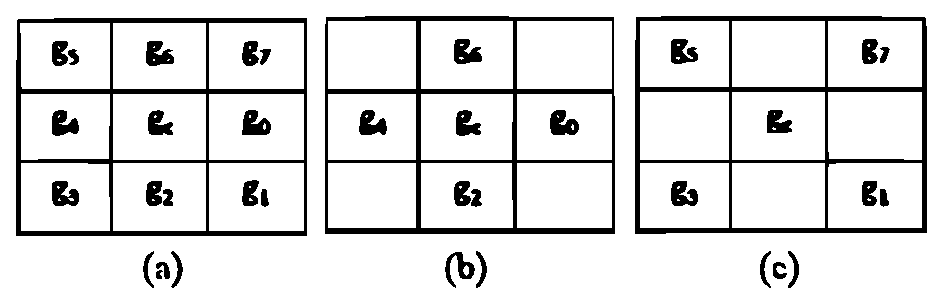
\includegraphics[height=3cm, width=8cm]{figureR1}
	\caption{\textbf{(a) Local region around $g_{c}$. (b) Nearest neighbours (c) Diagonal neighbours}}
\end{center}
\end{figure}
	
Following equation $(1)$ and $(2)$ represents the modified CSLBP for the nearest and the diagonal neighbours.
\begin{equation}
M-CSLBP_{N}(g_c)=s(g_0-g_4)2^1+s(g_2-g_6)2^2
\end{equation}
\begin{equation}
M-CSLBP_{D}(g_c)=s(g_1-g_5)2^1+s(g_3-g_7)2^2
\end{equation}
\begin{equation}
sign(g_p-g_{p+(P/4)})=\begin{cases}1 & (g_p-g_{p+(P/4)})>T\\0 & otherwise\end{cases}
\end{equation}
\\
where:\\
$T$ : non-negative value to extract texture for uneven surface;\\
$g_c$: center pixel;\\
$g_p$: neighbours of center pixel;\\
$P$: neighbours of center pixel $P=8$;\\
$g_{p+(P/4))}$: sign function of M-CSLBP;\\
$M-CLBP_N$: Modified CSLBP for the nearest neighbour;\\
$M-CLBP_D$: Modified CSLBP for the diagonal neighbour.\\


The pixel value varies from $0$ to $3$ for each neighbour in the modified CSLBP. In the modified CSLBP, like CSLBP all four cross-symmetric pairs are covered. But unlike the CSLBP,  all pairs are not combined in one histogram of $16$ bin. Instead, the two different histograms are generated, each of four bin by separating neighbours. The generated histogram of modified CSLBP is of $8$ bin which shows $50\%$ saving of hash code. Two weight factors, Standard deviation (SD) and Laplacian of Gaussian (LoG) are used for the nearest and the diagonal neighbours. SD weight factor is calculated from an original image while LoG weight factor is derived the Gradient image. 
\par
Standard deviation is one of the powerful texture descriptor. It represents average distance from the mean of the data set to a center point. Standard deviation is calculated for both the neighbours by following equations (4) and (5) respectively. For center pixel $g_c$, absolute difference of four cross-symmetric pairs are taken as ($g_0$-$g_4$), ($g_1$-$g_5$), ($g_2$-$g_6$) and ($g_3$-$g_7$). The nearest neighbour pairs are ($g_0$-$g_4$), ($g_2$-$g_6$) and the diagonal neighbour pairs are ($g_1$-$g_5$), ($g_3$-$g_7$).

%$\overline{g}=\frac{(g_{0}-g_{4})+(g_{2}-g_{6})}{2} \quad g_{i}=[(g_{0}-g_{4}),(g_{2}-g_{6})]$

\begin{equation}
SD_N=\sqrt{\frac{\sum_0^1(g_N-\overline{g_N})^2}{2}}
\end{equation}


\begin{equation}
\overline{g_{N}}=\frac{(g_{0}-g_{4})+(g_{2}-g_{6})}{2} 
\end{equation}


\begin{equation}
g_{N}=[(g_{0}-g_{4}),(g_{2}-g_{6})]
\end{equation}


\begin{equation}
SD_D=\sqrt{\frac{\sum_0^1(g_D-\overline{g_D})^2}{2}}
\end{equation}


\begin{equation}
\overline{g_{D}}=\frac{(g_{1}-g_{5})+(g_{3}-g_{7})}{2} 
\end{equation}

\begin{equation}
g_{D}=[(g_{1}-g_{5}),(g_{3}-g_{7})]
\end{equation}
where:\\
$SD_{N}$ and $SD_{D}$: Standard Deviation weight factor of the nearest and the diagonal neighbours respectively. 
\\
\par
The Laplacian of an image highlights regions of rapid intensity change and is therefore often used for edge detection. If Laplacian filter is applied directly on a noisy image, the result is an edge image with many small edges which are not more useful. The Laplacian is often applied to an image that has been smoothed first with a gaussian smoothing filter in order to reduce its sensitivity to noise. The LoG response will be zero for areas where the image has a constant intensity. However, in the vicinity of a change in intensity, the LoG response will be positive on the darker side, and negative on the lighter side. This indicates reasonably sharp edge between two regions of uniform but different intensities. The Laplacian of Gaussian filter detects the horizontal and vertical boundaries as well as the boundaries other than the horizontal and vertical ones. The $2D$ Laplacian of Gaussian (LoG) function centered on zero and with Gaussian standard deviation $sigma (\sigma)$ has the form:
\begin{equation}
LoG(x,y)=-\frac{1}{\pi\sigma^4}[1-\frac{x^2+y^2}{2\sigma^2}]e^-\frac{x^2+y^2}{2\sigma^2}
\end{equation}
where:\\
$\sigma$ : standard deviation;\\
x and y: spatial coordinates of an image.
\par
The amount of smoothing can be controlled by varying the value of the standard deviation. In proposed method, LoG of input image is calculated to the generate gradient image. Weight factor is determined by taking average of LoG gradient information of the nearest neighbours and the diagonal neighbours respectively. For example for pixel $G_c$ with $8$ gradient neighbours from $G_0$ to $G_7$.


\begin{equation}
LoG_{N}=\frac{(G_{0}+G_{2}+G_{4}+G_{6})}{4}
\end{equation}


\begin{equation}
LoG_{D}=\frac{(G_{1}+G_{3}+G_{5}+G_{7})}{4}
\end{equation}
where:\\
$LoG_{N}$ and $LoG_{D}$: LoG weight factor of the nearest and the diagonal neighbours respectively. \\
\\
Final weight for the nearest and the diagonal neighbours are given by equations $(9)$ and $(10)$.
\begin{equation}
W_{N}=SD_{N}+LoG_{N}
\end{equation}
\begin{equation}
W_{D}=SD_{D}+LoG_{D}
\end{equation}
where:\\
$W_{N}$ and $W_{D}$ : Weight factor of the nearest and the diagonal neighbours respectively. 
\par
After calculation of the modified CSLBP, histogram is constructed at sub-block level. The sub-block size is trade off between hash size and discrimination capability. For a large sub-block size, the resultant image hash size decreases. However, discrimination and local area forgery detection rate gets reduced. For every sub-block, two histogram are generated, each of a $4$ bin. While constructing the modified CSLBP histogram, particular histogram bin is not incremented by one like CSLBP histogram. However, bin is incremented by weight factor. Equation of the modified CSLBP histogram for the nearest and the diagonal neighbours are given as below.
\begin{equation}
H_{MCSLBP-N}=\sum_{i=1}^B\sum_{j=1}^BW_N \times f(M-CSLBP_{N}(i,j),b)
\end{equation}

\begin{equation}
H_{MCSLBP-D}=\sum_{i=1}^B\sum_{j=1}^BW_D \times f(M-CSLBP_{D}(i,j),b)
\end{equation}
where:\\
f: bin increment function;\\
$H_{MCSLBP-N}$: histogram for nearest neighbours; \\
$H_{MCSLBP-D}$: histogram for diagonal neighbours; \\
B: size of sub-block; \\
$b\epsilon[0,3]$. 
\par
If the image is manipulated maliciously, then weight factor of an original image and its modified version will not be the same. This difference captures perceptual characteristics of hashing. For content-preserving operations, image hash of an original and content-preserving modified image is different, still difference of hash codes remains within the prescribed limits of the set threshold. If the modified CSLBP histogram is constructed without weight factor then discrimination power which contributes in success rate is low. Histogram constrcuted with weight factor captures perceptualness at local level and identifies change area of an image.
\par
Uniform quantization is applied separately on each histogram to generate a binary hash. In uniform quantization, the step size between adjacent quantized levels is fixed. All the sub blocks are processed in this manner and quantized hash code of all sub blocks are concatenated to generate the final hash of the image. On the receiver side, binary hash can be efficiently compared with hamming distance. If hamming distance is less than the set threshold, then it is content-preserving manipulation, otherwise it is treated as content-change manipulation.

\section{Experimental Result Analysis}
In image hashing authentication, robustness to content-preserving and sensitivity to content-change are important properties to be evaluated. These two properties are evaluated using two benchmarks. One is Normalized hamming distance (NHD) and other is Receiver Operating Characteristics (ROC) are used. Above mentioned benchmarks are suitable for binary classification that is either authentic or non-authentic. NHD measures how much change happen for both content-preserving and content-change operations. ROC basically checks discrimination capability of hashing methods.

\subsection{Experimental Setup}
From original database, two database are created namely malicious and non-malicious. For analysis purpose, the total $36$ images are taken from Matlab directory and the internet. To compare performance with other methods, all images are set to uniform standard size $256\times256$. For every image, total $61$ attacks are applied as specified in Tabble 1. Some of the attacks are content-preserving while others are content-change. Table 2 specifics acronyms for various attacks. Table 3 specifies various comparative methods with their acronyms.
\par
Following paragraph describes various parameter used in the modified CSLBP calculation. Input image is divided into non overlapping sub-blocks of size $3\times3$ i.e. $R=1$ and $P=8$ which represent neighbour around center pixel. $T$ is non-negative threshold for texture extraction and it is set to $0.1$. The gradient image (G) is generated by applying LoG operator on input image. For LoG operator, $\sigma$ is $0.9$. For the histogram generation, sub-block size is set to $32\times32$. This sub-block size gives good balance between hash size and discrimination capability.

\begin{table} [h]
	\captionsetup[table]{skip=10pt,justification=centering}
	\caption{Various attacks with parameter}
	\centering
	
	\begin{tabular}{|p{2.9cm}|p{2.6cm}|p{6.9cm}|}
		\hline \textbf{Attacks} & \textbf{Detail} &  \textbf{Parameters} \\ 
		\hline Cropping	 & Ratio &	$1\%$, $3\%$, $5\%$, $7\%$, $9\%$  \\
		\hline Salt \& Pepper Noise & Density	& 0.01, 0.02, 0.03, 0.05, 0.1\\
		\hline Gaussian Noise &	Variance & 0.001, 0.005, 0.01, 0.02, 0.05\\
		\hline JPEG Compression	& Quality Factor & 10, 30, 50, 70, 90\\
		\hline Rotate &	Rotation Angle&	2$^{\circ}$, 4$^{\circ}$, 6$^{\circ}$, 8$^{\circ}$, 10$^{\circ}$ \\
		\hline Gamma  & Gamma Value	& 0.75, 0.8, 0.9, 1.1, 1.25  4.25, 4.50, 5.00, 5.25 \\
		\hline Scaling & Scaling Factor & 0.7, 0.8, 0.9, 1.1, 1.2, 0.01, 0.05, 0.10, 0.15, 0.20 \\
		\hline Increase Brightness & Range  &	[0.8 1], [0.6 1], [0.4 1], [0.2 1]\\
		\hline Decrease Brightness & Range  & [1 0.8], [1 0.6], [1 0.4], [1 0.2]\\
		\hline Increase Contrast & Range   & [0 0.8], [0 0.6], [0 0.4], [0 0.2]\\
		\hline Decrease Contrast & Range & [1 0.8], [1 0.6], [1 0.4], [1 0.2] \\
		\hline 
	\end{tabular} 
	\vspace{5mm}
	\captionsetup[table]{skip=10pt,justification=centering}
	%	\caption{VARIOUS ATTACKS AND THEIR INTENSITY }
	\caption{Attacks with their Acronym}
	\centering
	%https://books.google.co.in/books?id=c8_2LMURd3AC&pg=SA2-PA9&source=gbs_se%lected_pages&cad=2#v=onepage&q&f=false
	\begin{tabular}{|p{2.9cm}|p{1.4cm}|p{2.9cm}|p{1.4cm}|}
		\hline \textbf{Attack Name}	 &  \textbf{Acronym}  & \textbf{Attack Name}  &  \textbf{Acronym}\\ 
		\hline Cropping & A &   Salt \& Pepper & B \\ 
		\hline Gaussian & C &   Scaling & D \\ 
		\hline Rotation & E &   JPEG & F \\ 
		\hline Gamma Correction & G &   Brightness Plus & H \\ 
		\hline Brightness Minus & I &   Increase Contrast & J \\ 
		\hline Decrease Contrast & K &  Average of Database & Avg \\ 
		\hline 
	\end{tabular} 
	\vspace{5mm}
	\captionsetup[table]{justification=centering}
	\centering
	\caption{Methods with their Acronym}
	% {|c|c|c|} 
	\begin{tabular}{|p{3.9cm}|p{1.2cm}|p{6.3cm}|}
		\hline   \textbf{Attacks} &     \textbf{Acronym} &     \textbf{Weight Factor}  \\ 
		\hline  CSLBP                &  I    &    Only Sign \\ 
		\hline  CSLBP Sep. Mag. &  II   &    Separate Magnitude \\
		\hline  Q-CSLBP               &  III  &   Only Sign \\
		\hline  AQ-CSLBP              &  IV   &   \small Magnitude Average \\
		\hline  SDQ-CSLBP             &  V    &   \small Standard Deviation \\
		\hline  CoCQ-CSLBP            &  VI   &   \small Correlation Coefficient \\
		\hline LoGQ-CSLBP             &  VII  &   \small Laplacian of Gaussian \\
		\hline  Proposed Modified CSLBP      &  VIII &   \small Standard Deviation + Laplacian of Gaussian \\
		\hline 
	\end{tabular} 	
\end{table}


\subsection{Perceptual Robustness Test}
Perceptual robustness measure indicates content preserving. It ensures that original image and its attacked version are visually similar. It categorizes such type of modification as non-malicious operations and attack version is accepted as authentic image. To check for visual similarity, normalized hamming distance is used. Hamming distance is simple ex-or operation. Two hashes, one from original image and other from its attacks version is ex-ored to get hamming distance. Hamming distance is normalized for analysis simplicity. The threshold $T_{NHD}$ is set for Normalized Hamming Distance (NHD). For authentic image, NHD between original image and its attacked version is less than $T_{NHD}$ and for non-authentic images it is greater than the set threshold. $T_{NHD}$ for every method is different. For modified CLSBP, $T_{NHD}$ is $0.14$. The proposed method is compared with other existing methods from method I to VII as mentioned in Table 3. 

\begin{table}[h]
	%[!htbp]
	\centering
	%\tiny
	\caption{NHD for Method I: CSLBP(Sign), Method II: CSLBP (Sep. Mag.),
		Method III: Q-CSLBP}
	
	\begin{tabular}{*7c}
		
		\toprule
		
		Attack
		
		& \multicolumn{2}{c}{Method I} 
		& \multicolumn{2}{c}{Method II}
		& \multicolumn{2}{c}{Method III}
		
		
		\\
		\midrule
		
		{}   &  Auth.  &  Non Auth.  &  Auth.  &  Non Auth.  & Auth.  &  Non Auth.   \\
		% &  Auth.  &  Non Auth.  & Auth.  &  Non Auth.   & Auth.  &  Non Auth. 
		
		
		
		A	& 0.04	& 0.10	& 0.01	& 0.01	& 0.05	& 0.13   \\
		
		B	& 0.03	& 0.11	& 0.01	& 0.01	& 0.04	& 0.10   \\
		
		C	& 0.14	& 0.22	& 0.01	& 0.02	& 0.12	& 0.19   \\
		
		D	& 0.02 	& 0.14	& 0.00	& 0.02	& 0.02	& 0.17   \\
		
		E	& 0.05 	& 0.10	& 0.01	& 0.01	& 0.07   & 0.13   \\
		
		F	& 0.03 	& 0.09	& 0.00	& 0.01	& 0.03   & 0.10   \\
		
		G	& 0.01 	& 0.12	& 0.00	& 0.01	& 0.01   & 0.13   \\
		
		H	& 0.04 	& 0.12	& 0.00	& 0.01	& 0.05	& 0.14   \\
		
		I	& 0.03 	& 0.18	& 0.00	& 0.02	& 0.03	& 0.21   \\
		
		J	& 0.05 	& 0.17	& 0.01	& 0.02	& 0.06	& 0.20   \\
		
		K	& 0.04 	& 0.16	& 0.00	& 0.02	& 0.04	& 0.19  \\
		
		\bottomrule
	\end{tabular}
\end{table}

Table 4. clearly shows that method 1 and method III satisfies perceptual robustness. Method I is implemented CSLBP texture operator and generates 16 bin histogram. Method III is same as method I only histogram is compressed from 16 bin to 18 bin using the flipped difference concept. Method II is implemented by author Davarzani\cite{davarzani2015}. has poor perceptual property as it fails to distinguished between content-change and content-preserving. This method used weight factor as magnitude of difference of cross-symmetric pairs of CSLBP. For each pair, they generate separate histogram of 16 bin. This results in histogram 64 bin and subsequently increase resultant hash size. \\


\begin{table} [h]
	%[!htbp]
	\centering
	%\tiny
	
	
	
	\caption{NHD for Method IV: AQ-CSLBP,  V:SDQ-CSLBP, Method VI: CoCQ-CSLBP Method VI: LoGQ-CSLBP}	
	\begin{tabular}{*9c}
		
		\toprule
		
		Attack
		
		& \multicolumn{2}{c}{  Method IV} 
		& \multicolumn{2}{c}{  Method V}
		& \multicolumn{2}{c}{  Method VI}
		& \multicolumn{2}{c}{  Method VII}
		
		
		
		\\
		\midrule
		
		{}   & Auth  & Non  Auth.  & Auth  &  Non  Auth.  &  Auth  & Non Auth.  & Auth.  & Non Auth. \\
		%A    &\footnotesize .86   & .86    & .08  & .81  & .08  & .81    \\
		
		A  & 0.04	 & 0.11	 & 0.05	 & 0.13	 & 0.05	 & 0.13   & 0.06 & 0.14 \\	
		
		B  & 0.06   & 0.12  & 0.07  & 0.15  & 0.04  & 0.10   & 0.05 & 0.11 \\	
		
		C  & 0.09	 & 0.14	 & 0.11	 & 0.19	 & 0.13	 & 0.17   & 0.12 & 0.19 \\	
		
		D  & 0.02	 & 0.17	 & 0.02	 & 0.19	 & 0.02	 & 0.19   & 0.03 & 0.19 \\	
		
		E  & 0.07	 & 0.13	 & 0.09	 & 0.15	 & 0.07	 & 0.13   & 0.08 & 0.15 \\	
		
		F  & 0.02	 & 0.07	 & 0.02	 & 0.08	 & 0.04	 & 0.13   & 0.04 & 0.09 \\	
		
		G  & 0.01	 & 0.14	 & 0.01	 & 0.16	 & 0.02	 & 0.16   & 0.01 & 0.12 \\	
		
		H  & 0.05	 & 0.15	 & 0.05	 & 0.17	 & 0.06	 & 0.17   & 0.04 & 0.11 \\	
		
		I  & 0.03	 & 0.27	 & 0.03	 & 0.30	 & 0.04	 & 0.26   & 0.03 & 0.18 \\	
		
		J  & 0.04	 & 0.18	 & 0.04	 & 0.20	 & 0.08	 & 0.26   & 0.04 & 0.15 \\	
		
		K  & 0.04	 & 0.20	 & 0.04	 & 0.21	 & 0.06	 & 0.24   & 0.04 & 0.18 \\	
		
		\bottomrule
		
		% A	0.04	0.11	0.05	0.13	0.05	0.13	0.06	0.14
	\end{tabular}
	
\end{table}


Table 5 represents our previous approaches in which we achieved perceptual robustness as well as discrimination capability. Method IV to VII, all are generated 8 bin histogram using the flipped difference concept. However flipped difference concept compresses histogram but its overall discrimination power is low. To enhance this discrimination power, various weight factors are utilized during CSLBP construction. 
\par 
Table 6 shows normalized hamming distance for the proposed modified CSLBP. $T_{NHD}$ is set to $0.14$. It clearly shows that method successfully distinguished between malicious and non-malicious operations. Proposed method fail to distinguish only malicious operations by JPEG attack. Larger value of the normalized hamming distance is, the higher is the discrimination capability. Figure. 2 shows graphical representation of NHD for the proposed method. From the above graph it is clear that the proposed method is quite robust for all types of attacks.
\begin{table}[h]
	%[!htbp]
	\centering
	\caption{NHD for Modified CSLBP}
	\footnotesize
	\centering
	\begin{tabular}{*3c}
		
		\toprule
		
		Attack
		
		&  \multicolumn{2}{c}{Modified CSLBP} 
		\\
		\midrule
		{}   &  Auth.  &  Non Auth.       \\
		%A    &\footnotesize .86   & .86    & .08  & .81  & .08  & .81    \\
		A	& 0.07	& 0.16 \\
		B	& 0.06	& 0.16 \\
		C	& 0.13	& 0.23 \\
		D	& 0.03	& 0.24 \\
		E	& 0.11	& 0.18 \\
		F	& 0.03	& 0.09 \\
		G	& 0.02	& 0.19 \\
		H	& 0.06	& 0.19 \\
		I	& 0.04	& 0.31 \\
		J	& 0.05	& 0.23 \\
		K	& 0.05	& 0.25 \\
		\bottomrule
	\end{tabular}
\end{table}
\begin{figure}
	\centering
	\includegraphics[width=80mm, height=45mm]{NHDproposedmethod.png}
	%	\label{fig3}
	\caption{\textbf{Graphical representation of NHD for Modified CSLBP}}
\end{figure}

\subsection{Discrimination Test}
Receiver Operator Characteristic (ROC) curve is used to display the performance of a binary classification algorithms at various threshold settings. TPR and FPR indicate robustness and discrimination, respectively. The area under the ROC curve is a measure of how well a parameter can distinguish between two diagnostic groups (authentic/non-authentic). Accuracy is measured by the area under the ROC curve. An area of 1 represents a perfect test; an area of 0.5 represents a worthless test. ROC curve is obtained by plotting TPR and FPR on Y and X axis respectively, for a Figure 3 shows respective graphical representation.

\begin{table}[h]
	%[!htbp]
	\centering
	
	\footnotesize
	%\tiny
	%	\small
	
	\centering
	\begin{tabular}{*3c}
		
		\toprule
		
		Attack
		
		&  \multicolumn{2}{c}{ Modified CSLBP} 
		
		
		\\
		\midrule
		{}   &  TPR  &  FPR       \\
		%A    &\footnotesize .86   & .86    & .08  & .81  & .08  & .81    \\
		
		
		A	& 0.90	& 0.06 \\
		B	& 0.90	& 0.25 \\
		C	& 0.47	& 0.07 \\
		D	& 1.00	& 0.07 \\
		E	& 0.44	& 0.05 \\
		F	& 0.99	& 0.67 \\
		G	& 1.00	& 0.08 \\
		H	& 0.85	& 0.03 \\
		I	& 1.00	& 0.01 \\
		J	& 0.88	& 0.10 \\
		K	& 0.94	& 0.19 \\
		Avg.& 0.89  & 0.11 \\  
		\bottomrule
	\end{tabular}
	\caption{ROC for Modified CSLBP}
	
\end{table}


\begin{figure}
	\centering
	\includegraphics[width=80mm, height=45mm]{ROCproposedmethod.png}
	%	\label{fig3}
	\caption{\textbf{ROC for Modified CSLBP}}
\end{figure}

For an average database, TPR is 0.89. If weight factor is not utilized, then TPR is close to 0.82, which shows that with the help of local weight factor, the discrimination power of hashing algorithm can be enhanced. ROC results for methods I to VIII are represented in Figure from 4-15. Method I to VII are comparative methods while method VIII is proposed method. From Figure 4 to 14, it shows that the proposed modified CSLBP is quite robust for almost all types of attack with good discrimination capability. Only for decrease contrast and JPEG quality factors, performance is average.

%Tables and Figures are presented center, as shown below and cited in the manuscript.\\

\begin{figure}[h]
	\begin{multicols}{2}
		\includegraphics[width=\linewidth]{1cropping.png}\par\caption{ROC: Cropping}
		\includegraphics[width=\linewidth]{2saltandpepper.png}\par\caption{ROC: Salt \& Pepper Noise}
		
	\end{multicols}
\end{figure}

\begin{figure}[h]
	\begin{multicols}{2}
		\includegraphics[width=\linewidth]{3gaussian.png}\par\caption{ROC: Gaussian Noise}
		\includegraphics[width=\linewidth]{4scaling.png}\par\caption{ROC: Scaling}
		
	\end{multicols}
\end{figure}

\begin{figure}[h]
	\begin{multicols}{2}
		\includegraphics[width=\linewidth]{5rotation.png}\par\caption{ROC: Rotation}
		\includegraphics[width=\linewidth]{6jpeg.png}\par\caption{ROC: JPEG}
		
	\end{multicols}
\end{figure}

\begin{figure}[h]
	\begin{multicols}{3}
		\includegraphics[width=\linewidth]{7gammacorrection.png}\par\caption{ROC: Gamma Correction}
		\includegraphics[width=\linewidth]{8increasebrightness.png}\par\caption{ROC: Increase Brightness}
		\includegraphics[width=\linewidth]{9decreasebrightness.png}\par\caption{ROC: Decrease Brightness}
		
	\end{multicols}
\end{figure}

\begin{figure}[h]
	\begin{multicols}{2}
		\includegraphics[width=\linewidth]{10increasecontrast.png}\par\caption{ROC: Increase Contrast}
		\includegraphics[width=\linewidth]{11decreasecontrast.png}\par\caption{ROC: Decrease Contrast}
	\end{multicols}
\end{figure}




From figure 4 to 14, it shows that the proposed modified CSLBP is quite robust for almost all types of attack with good discrimination capability. Only for decrease contrast and JPEG quality factors, performance is average.    



\section{Conclusion}

We have proposed the modified CSLBP image hashing method with weight factor. Loss is more when quantization is applied on long histogram. Also long histogram increases resultant image hash size. To overcome these problems, small histogram are generated for different neighbours. Advantage with small histogram is hash size decreases by $50\%$  and there is less loss on quantization. Discrimination power is enhanced by local weight factor namely, standard deviation and LoG. Compact length and desirable discrimination power are two main characteristics of hashing are achieved by proposed method. Proposed method is robust to variety types of attacks as results are proved by NHD and ROC curve.
	
	\begin {thebibliography}{99}
	
		%1. conference
		\bibitem{mall2012}
		V. Mall, K. Bhatt, S. ~K. Mitra and A.~K. Roy, Exposing structural tampering in digital images, {\em Proc. of the Int'l Conference on Sinal Processing, Computing and Control (ISPCC)}, Solan, India, pp.1--6, 2012.
		
		
		%2. conference
		\bibitem{mall2013}
		V. Mall, S. Shukla, S. ~K. Mitra and A.~K. Roy, Comprehensive image index and detection of tampering in a digital image, {\em Proc. of the 2nd Int'l Conference on Informatics, Electronics and Vision (ICIEV 2013)}, Dhaka, Bangladesh, pp.1--7, 2013.
		
		
		%3 conference
		\bibitem{mallroy2013}	
		V. Mall, A.~K. Roy and S. ~K. Mitra, Digital image tampering detection and localization using singular value decomposition technique, {\em Proc. of the 4th Int'l Conference on Computer vision, pattern recognition, image processing and graphics (NCVPRIPG)}, Jodhpur, India, pp.1--4, 2013.
		
		
		
		 % 4 IEEE Transaction
		 \bibitem{zhao2013} 
	 	Y. Zhao, S. Wang, X. Zhang and H. Yao,
		Robust hashing for image authentication using Zernike moments and local features, {\em Information Forensics and Security}, vol.8, no.1, pp.55--63, 2013.
		
		%5 Springer Conference
		\bibitem{soman2016}
		G. Soman and J. ~K. John,
		Block-Based Forgery Detection Using Global and Local Features {\em Proc. of the Int'l Conference on Soft Computing Systems}, Springer, New Delhi, India, pp. 147--155, 2016.
		
		
		% 6 Elsevier Conference
		\bibitem{sebastian2015}	
		L. ~S. Sebastian, A. Varghese and T. Manesh, Image authentication by content preserving robust image hashing using local and global features, {\em Proc. of the Int'l Conference on Information and Communication Technologies (ICICT 2014)}, Procedia Computer Science, 46, pp. 1554--1560, 2015.
		
		
		
		% 7 IEEE Conference
		\bibitem{neelima2015}	
		A. Neelima and K. ~M. Singh,
		A robust image hash function based on color and texture features of the image, {\em Proc. of the Int'l Conference on Advanced Computing and Communication (ISACC)}, Silchar, India, pp.238--243, 2015.
		
				
			
		% 8
		\bibitem{lei2010}
		Y. ~Q. Lei, K. ~Y. Chau, Z. ~M. Lu and W. ~H. Ip,
		DCT-domain global feature and DWT-domain least-squares line fitting based local feature for robust image hashing, {\em International Journal of Innovative Computing, Information and Control}, vol.6, no.6, pp.450--464, 2010., vol.6, no.6, pp.450--464, 2010.
		
		
		
		% 9 Journal 
		\bibitem{karsh2016}
		R. ~K. Karsh, R. ~H. Laskar and B. ~B. Richhariya, Robust image hashing using ring partition-PGNMF and local features, {\em SpringerPlus}, vol. 5, no. 1, pp. 1995, 2016.
		 
		 
		% 10 Journal 
		\bibitem{karsh2017}
		R. ~K. Karsh and R. ~H. Laskar,
		Robust image hashing through DWT-SVD and spectral residual method, {\em EURASIP Journal on Image and Video Processing}, vol. 1, no. 1, pp. 31, 2017.
		
		
		% 11 Journal 
		\bibitem{yuling2016}
		L. ~I. ~U. Yuling, X. ~I. ~N. Guojiang, X. ~I. ~A. ~O. Yong, Robust Image Hashing Using Radon Transform and Invariant Features, {\em Radioengineering}, vol. 25, no. 3, pp. 556-564, 2016.
		
		
		
		%12 IEEE Transaction
		\bibitem{monga2007} 
		V. Monga, Robust and secure image hashing via non-negative matrix factorizations, 	{\em Information Forensics and Security}, vol. 2, no. 3, pp. 376-390, 2007.
		
		
				
		% 13 Journal
		\bibitem{tang2008}
		Z. Tang, S. Wang, X. Zhang, W. Wei, S. Su, Robust image hashing for tamper detection using non-negative matrix factorization, {\em Journal of Ubiquitous Convergence Technology}, vol. 2, no. 1, pp. 18-26, 2008.
		
		
			
		% 14 IEEE Conference
		\bibitem{prungsinchai2013a}
		S. Prungsinchai, F. Khelifiet and A. Bouridane, Fourier-Mellin transform for robust image hashing, {\em Proc. of the 4th Int'l Conference on Emerging Security Technologies}, Cambridge, UK, pp. 58--61, 2013.
		
		
	
		%15 IEEE Transaction
		\bibitem{lu2012} 
		X. Lu and Z. J. Wang, Perceptual image hashing based on shape contexts and local feature points, {\em Information Forensics and Security}, vol. 7, no. 3, pp. 1081-1093, 2012.
		

		%16 IEEE Conferance
		\bibitem{yan2015}	
		C. Yan, C. Pun and X. Yuan, Adaptive local feature based multi-scale image hashing for robust tampering detection, {\em Proc. of the 10th Int'l Region Conference (TENCON)}, Macao, China, pp. 238--243, 2015.


		%17 IEEE Conferance
		\bibitem{sun2011}	
		R. Sun, W. Zeng and X. Yen,
		Perceptual Image Hashing Method Using Contourlet HMT Model, {\em Proc. of the 3rd Int'l Region Conference on Multimedia Information Networking and Security}, Shanghai, China, pp. 292--296, 2011.
		
		
		%18 Springer Conference
		\bibitem{guo2007}	
		X. ~C. Guo and D. Hatzinalos, Content based image hashing via wavelet and radon transform, {\em Proc. of the Pacific Rim Conference on Multimedia} Berlin/Heidelberg/New York, Springer, pp.755--764, 2007.
		
		
		%19 IEEE Conferance
		\bibitem{prungsinchai2013b}	
		S. Prungsinchai, F. Khelifiet and A. Bouridane, A DCT sign-based robust image hashing,
		{\em Proc. of the 8th Int'l Conference on Internet Technology and Secured Transactions, (ICITST-2013)}, London, UK, pp. 401-405, 2013.
	
	
		%20 IEEE Conferance
		\bibitem{srivastava2016}	
		M. Srivastava, J. Siddiqui, M.~A. Ali, Robust image hashing based on statistical features for copy detection, {\em Proc. of the Int'l Conference on Electrical, Computer and Electronics Engineering (UPCON)}, Varanasi, India, pp. 490-495, 2016.
	
	
		%21 IEEE Conferance
		\bibitem{ojala2002} 
		T. Ojala, M. Pietikainen and T. Maenpaa, Multiresolution gray-scale and rotation invariant texture classification with local binary patterns, {\em Pattern Analysis and Machine Intelligence}, vol. 24, no. 7, pp. 971-987, 2002.
		
		
		
		%22 IEEE Confereance
		\bibitem{xiao2011}	
		J. Xiao and G. Wu, A robust and compact descriptor based on Center-Symmetric LBP,	{\em Proc. of the 6th Int'l Conference on Image and Graphics (ICIG)}, Hefei, Anhui, China, pp. 388-393, 2011.
		
		%23 Journal
	    \bibitem{davarzani2015}
	    R. Davarzani, S. Mozaffari and K. Yaghmaie, Image authentication using LBP-based perceptual image hashing, Journal of AI and Data Mining, vol. 3, no. 1, pp. 22-30, 2015.	
	   
	    % 24
	    \bibitem{patil2016a}
	    V. Patil and T. Sarode, Image hashing using AQ-CSLBP with double bit quantization, {\em Proc. of the Int'l Conference on Optoelectronics and Image Processing}, Warsaw, Poland, pp. 30-34, 2016.
	    			
		% 25
		\bibitem{patil2016b}
		V. Patil and T. Sarode, Image hashing by SDQ-CSLBP, {\em Proc. of the Int'l Conference on Advances in Computing, Communications and Informatics ICACCI}, Jaipur, India, pp. 2057-2063, 2106.
		
		
		%26
		\bibitem{patil2016c}
		V. Patil and T. Sarode, Image hashing by CCQ-CSLBP, {\em Proc. of the Int'l Conference on Electrical and Computer Engineering, WIECON-ECE}, Pune, India, pp. 73-78, 2016.
		
		
		% 27
		\bibitem{patil2016d}
		V. Patil and T. Sarode, Image hashing by LoGQ-CSLBP, {\em Proc. of the Int'l Conference on on Communication and Information Processing}, Singapore, pp. 124-128, 2016.	
		
		
		% 28
		\bibitem{baber2012}
		J. Baber, S. ~I. Satoh, N. Afzulpurkar and M. Bakhtyar,
		Q-CSLBP: compression of CSLBP descriptor,
		{em\ Proc. of the Pacific Rim Conference on Multimedia}
		Berlin/Heidelberg/New York, Springer, pp.513--521, 2012.
		
	
	
\end{thebibliography}



\end{document}


